\documentclass[xcolor=dvipsnames]{beamer}
\usetheme{Rochester}
\usepackage{graphicx}
\usecolortheme[named=OliveGreen]{structure}
\useinnertheme{rounded}
\setbeamertemplate{blocks}[rounded][shadow=false]
\setbeamertemplate{items}[ball]
\begin{document}

\begin{frame}
    \frametitle{Netsoc Git Tutorial}

    \begin{center}
        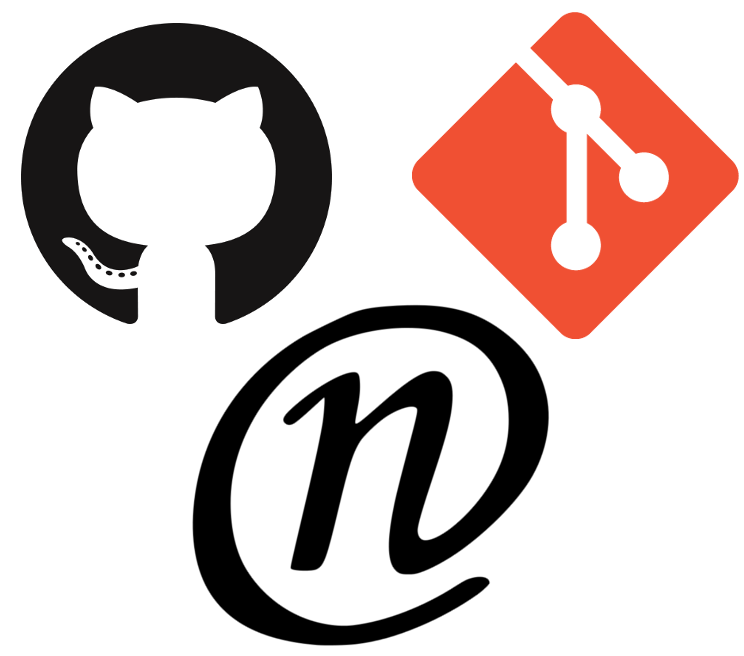
\includegraphics[scale=0.3]{nat.png}\\
        Slides by Tom Mason, Colm Vize and Andrew Anderson
    \end{center}
\end{frame}

\begin{frame}
    \frametitle{What is a VCS}
    
    Stands for Version Control System.\\
    A system used to control collaborative projects, so that multiple people can work on it at the same
    time without conflicts (as far as possible).\\
    Git is a DVCS, or Distributed CVS. This means that every user has a full copy of the project history.\\
\end{frame}

\begin{frame}
    \frametitle{Quick Glossary}
    "Working Directory" - The floder with your code in it, that you can edit\\
    "commit" - a set of changes to your repository that can be used to bring it from one state to another\\
    "push" - sending a bunch of commits somewhere\\
    "pull" - grabbing a bunch of commits from somewhere
\end{frame}

\begin{frame}
    \frametitle{What is github?}

    Github is a hosting site for open source projects using git as their VCS\\
    Has a nice WebUI\\
    Streamlined Pull requests (more on this later)\\
\end{frame}

\begin{frame}
    \frametitle{Create a github repo}

    Create a github accont (duh)\\
    Create repo (initialise with readme so we can clone it)
    \begin{center}
        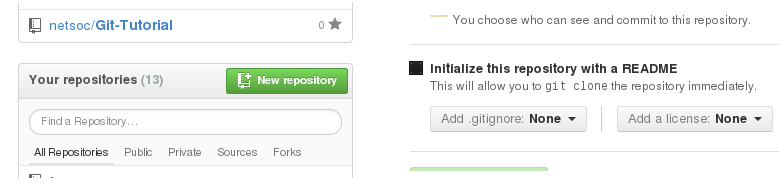
\includegraphics[scale=0.4]{gh-create-repo.png}
    \end{center}

\end{frame}

\begin{frame}
    \frametitle{Creating local repositories}

    You can also create a new repo locally by doing:
    \begin{block}{}
        mkdir myrepo\\
        cd myrepo\\
        git init
    \end{block}
    However, this will have no "remote", so you wan't be able to "push" it anywhere until you add some (more on this later)
\end{frame}

\begin{frame}
    \frametitle{Cloning repositories}
    Makes a local copy of a repository, from e.g github\\
    Works with lot of protocols (http, ssh, native git protocol, even local files).

    \begin{block}{Clone a local repository}
        git clone /path/to/repo
    \end{block}
    \begin{block}{Clone a remote repository (These slides!)}
        git clone https://github.com/username/your-repo.git
    \end{block}
\end{frame}

\begin{frame}
    \frametitle{Make your changes}
    After the cloning a repo, as on the previous slides, you will have a folder with the repositories
    files in it (normally source code for a program).

    Make your changes, and then...
\end{frame}

\begin{frame}
    \frametitle{Add and commit}
    Commit them.
    You can stage chages (select them for committing) by using
    \begin{block}{}
        git add $\langle$filename$\rangle$ \# adds $\langle$filename$\rangle$\\
        git add . \# also works on directories
    \end{block}
    To actually commit these changes use
    \begin{block}{}
        git commit -m "Commit message"
    \end{block}
    commits the changes we have added, with the message "Commit Message"\\
    
    \begin{block}{}    
        git commit
    \end{block}
     If you don't specify -m "whatever", git will open a text editor, and you can type your commit message in there 
    Now the file is committed to your local repo, but not on the remote repo \emph{yet}.
\end{frame}

\begin{frame}
    \frametitle{Remote repositories}

    You now have a commit in your local repository that isn't in the remote repository.
    You "push" this to the remote using
    \begin{block}{}
        git push origin master
    \end{block}
    
    origin is the name that git gives to the place you cloned a repository from.\\
    master is a branch, I will explain that later.

\end{frame}

\begin{frame}
    \frametitle{Pulling}

    Two copies of the repo (desktop + laptop, say)\\
    Make changes, commit and push on desktop\\\vbox{}
    What happens to the laptop copy? We use
    \begin{block}{}
        git pull
    \end{block}
    Pulls down all commits on the remote repo
\end{frame}

\begin{frame}
    \frametitle{Forking on github}

    On github, users can "fork" eachother's repos\\
    This creates a copy of that user's repo on your account\\

    \begin{center}
        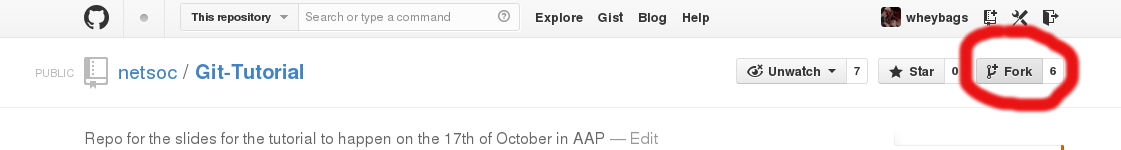
\includegraphics[scale=0.3]{gh-fork.png}
    \end{center}

    You then clone the repo from the copy on your account
\end{frame}

\begin{frame}
    \frametitle{Making Pull requests}

    If you want the original repo owner to pull in some changes from your repo\\
    Push to your repo, pull request from the webui

    \begin{center}
        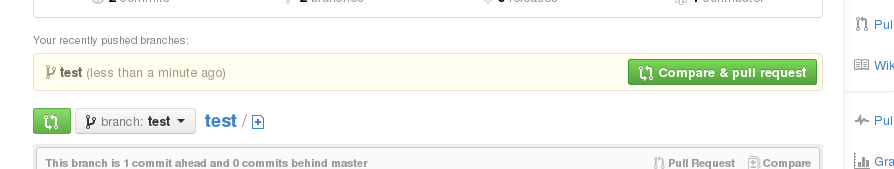
\includegraphics[scale=0.4]{gh-pullrequest.png}
    \end{center}

    Enter title, description etc
\end{frame}

\begin{frame}
    \frametitle{Merging pull requests}

    The sidebar on the original repo owner's page will show a new pull request\\
    They can click and use the webui to merge, or they can do it the traditional way with the command line (github has help built in to the page for this)

    \begin{center}
        
\includegraphics[scale=0.4]{gh-mergepullrequest.png}
    \end{center}
\end{frame}

\begin{frame}
    \frametitle{Branches}
    
    Like a local fork, within your own copy of the repo\\
    "master" from before, is just the main, default branch\\
    Often used to make branch for a feature\\
    Merged into master when feature is done\\
\end{frame}

\begin{frame}
    \frametitle{Branches}

    To create a local branch called testbranch
    \begin{block}{}
        git checkout -b testbranch
    \end{block}
    This will create the branch based on your current branch (master), and switch into it\\

    To view branches
    \begin{block}{}
        git branch
    \end{block}
    The current branch will have an asterix beside it

    To change back to branch master
    \begin{block}{}
        git checkout master
    \end{block}
\end{frame}

\begin{frame}
    \frametitle{Branches}
        Edit a file on the new branch and commit it\\
        Then git checkout master\\
        Your changes will have vanished because they are committed to the other branch\\
        You can "merge" in changes from a branch into current branch with
        \begin{block}{}
            git merge testbranch
        \end{block}
\end{frame}

\begin{frame}
    \frametitle{Conflicts}

    What happens if we try to merge or pull and there are conflicts?\\\vbox{}
    
    This is called a merge conflict\\
    Git resolves simple merge conflicts automagically\\
    Sometimes, we have to do it manually\\
\end{frame}

\begin{frame}
    \frametitle{Merge Conflicts}

    For example, user1 makes repo with file "test" saying "i am a test"\\
    user2 clones repo\\
    user1 chages to "i are a test", commits, pushes\\
    user2 changes to "i am not a test", commits, pulls\\

    user2 will then get this error:
    \begin{center}
        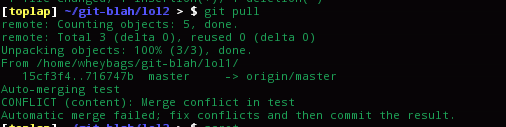
\includegraphics[scale=0.4]{mergeconflict1.png}
    \end{center}
\end{frame}

\begin{frame}
    \frametitle{Merge conflicts}

    git status shows what files you need to fix

    \begin{center}
        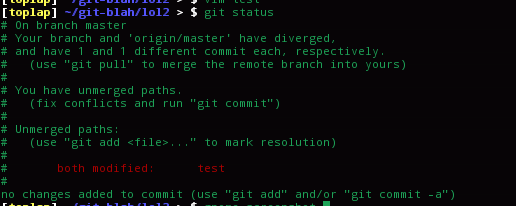
\includegraphics[scale=0.4]{mergeconflict2.png}
    \end{center}
\end{frame}
 
\begin{frame}
    \frametitle{Merge conflicts}

    Edit the file, and see the section git can't fix

    \begin{center}
        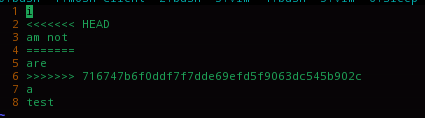
\includegraphics[scale=0.4]{mergeconflict3.png}
    \end{center}

    Then fix it manually

    \begin{center}
        
\includegraphics[scale=0.4]{mergeconflict4.png}
    \end{center}

    Between $<<<<<$ and ===== is user1's version, between ==== and $>>>>>$ is user2's
\end{frame}


\begin{frame}
    \frametitle{Merge conflicts}

    git add to mark the file as fixed, then git status will show it in green

    \begin{center}
        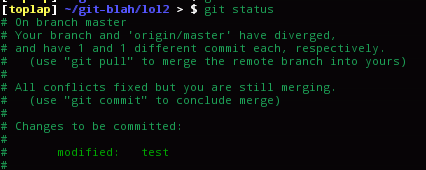
\includegraphics[scale=0.4]{mergeconflict5.png}
    \end{center}

    Then just commit and push as normal\\
    Often git will auto merge things, so long as they're not in the same part of the same file
\end{frame}

\begin{frame}
    \frametitle{Remotes}

    When you clone, a default "remote" is created, origin\\
    So "git push origin master" means "push the default branch to the place I got this from"\\
    You can add multiple remotes\\
    This is useful for other people's forks
\end{frame}

\begin{frame}
    \frametitle{Remotes}
    Tell git where to get jonnosfork
    \begin{block}{}
        git remote add jonnosfork https://github.com/jonno/myrepo.git
    \end{block}

    Download the changes Jonno has made (this won't override your stuff)
    \begin{block}{}
        git fetch jonnosfork     
    \end{block}
    
    Then you can "git merge jonnosfork/master"\\
    Can also push to remotes if you have permission eg "git push jonnosfork master"
\end{frame}

\begin{frame}
    \frametitle{Stashes}
    
    Sometimes want to pull, merge, etc when not finished with a commit\\
    "git stash" saves uncommitted changes to a stack of stashes, and remove the from your working dir\\
    "git stash pop" will apply the changes like a merge to your working dir and remove from stack\\
\end{frame}

\begin{frame}
    \frametitle{Fin}

     That is 99\% of what you need to know\\
     Great resource: http://git-scm.com/\\
     Latex source for slides available here: https://github.com/netsoc/Git-Tutorial\\
     Enjoy using git!
\end{frame}

\end{document}
